\documentclass[10pt]{article}
\usepackage[top=1.3cm,bottom=1.3cm,left=1.5cm,right=1.5cm]{geometry}
\usepackage{graphicx}
\usepackage{tikz}
\usetikzlibrary{shapes.geometric,arrows.meta,positioning}
\usepackage[T1]{fontenc}

\pagestyle{empty}
\setlength{\parindent}{0pt}

\tikzset{
  startend/.style={rectangle, rounded corners=6pt, draw=black, minimum width=3.1cm, minimum height=0.7cm, align=center, font=\scriptsize},
  proc/.style={rectangle, rounded corners=2pt, draw=black, thick, minimum width=3.1cm, minimum height=0.85cm, align=center, font=\scriptsize, inner sep=2pt},
  proccond/.style={proc, dashed},
  dec/.style={diamond, draw=black, thick, aspect=2.2, minimum width=2.6cm, minimum height=1.0cm, align=center, font=\scriptsize, inner sep=1pt},
  arr/.style={-{Latex[length=2mm]}, draw=black},
}

\begin{document}
\thispagestyle{empty}

\noindent
\begin{minipage}[t]{0.48\linewidth}
\centering
\resizebox{\linewidth}{!}{%
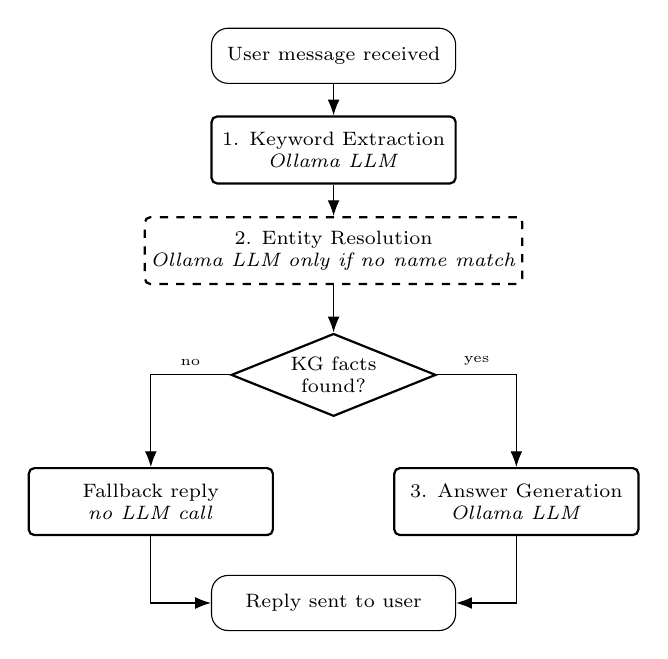
\begin{tikzpicture}[node distance=4mm and 3mm]
\node[startend] (n0) {User message received};
\node[proc, below=of n0] (n1) {1. Keyword Extraction\\\textit{Ollama LLM}};
\node[proccond, below=of n1] (n2) {2. Entity Resolution\\\textit{Ollama LLM only if no name match}};
\node[dec, below=6mm of n2] (n3) {KG facts\\found?};
\node[proc, below left=9mm and 1mm of n3] (n4l) {Fallback reply\\\textit{no LLM call}};
\node[proc, below right=9mm and 1mm of n3] (n4r) {3. Answer Generation\\\textit{Ollama LLM}};
\node[startend, below=20mm of n3] (n5) {Reply sent to user};
\draw[arr] (n0) -- (n1);
\draw[arr] (n1) -- (n2);
\draw[arr] (n2) -- (n3);
\draw[arr] (n3.west) -| node[pos=0.25,above,font=\tiny]{no} (n4l);
\draw[arr] (n3.east) -| node[pos=0.25,above,font=\tiny]{yes} (n4r);
\draw[arr] (n4l.south) |- (n5.west);
\draw[arr] (n4r.south) |- (n5.east);
\end{tikzpicture}%
}
\par\vspace{2pt}
\footnotesize\textbf{Fig.~1 --- LLM calls in the pipeline.} One model plays different roles in a single query; dashed boxes are conditional, solid boxes always run.
\end{minipage}
\hfill
\begin{minipage}[t]{0.48\linewidth}
\centering
\resizebox{\linewidth}{!}{%
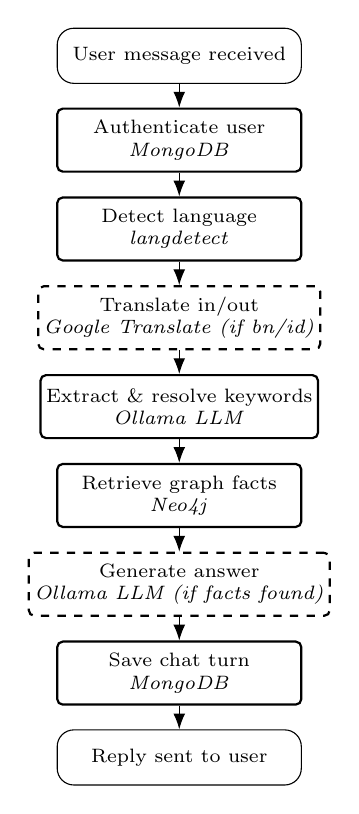
\begin{tikzpicture}[node distance=3mm, every node/.style={font=\scriptsize}]
\node[startend] (t0) {User message received};
\node[proc, below=of t0, minimum height=0.8cm] (t1) {Authenticate user\\\textit{MongoDB}};
\node[proc, below=of t1, minimum height=0.8cm] (t2) {Detect language\\\textit{langdetect}};
\node[proccond, below=of t2, minimum height=0.8cm] (t3) {Translate in/out\\\textit{Google Translate (if bn/id)}};
\node[proc, below=of t3, minimum height=0.8cm] (t4) {Extract \& resolve keywords\\\textit{Ollama LLM}};
\node[proc, below=of t4, minimum height=0.8cm] (t5) {Retrieve graph facts\\\textit{Neo4j}};
\node[proccond, below=of t5, minimum height=0.8cm] (t6) {Generate answer\\\textit{Ollama LLM (if facts found)}};
\node[proc, below=of t6, minimum height=0.8cm] (t7) {Save chat turn\\\textit{MongoDB}};
\node[startend, below=of t7] (t8) {Reply sent to user};
\draw[arr] (t0)--(t1);
\draw[arr] (t1)--(t2);
\draw[arr] (t2)--(t3);
\draw[arr] (t3)--(t4);
\draw[arr] (t4)--(t5);
\draw[arr] (t5)--(t6);
\draw[arr] (t6)--(t7);
\draw[arr] (t7)--(t8);
\end{tikzpicture}%
}
\par\vspace{2pt}
\footnotesize\textbf{Fig.~2 --- External tools invoked per query.}
\end{minipage}

\end{document}
